\documentclass[tikz,border=2pt]{standalone}
\usepackage{amsmath}
\usepackage{pgfplots}
\pgfplotsset{compat=1.18}
\begin{document}
% x'' + 3x' + 2x = 4t, x(0) = x'(0) = 0: x(t) = x_p(t) + (4e^{-t} - e^{-2t}) with x_p(t) = 2t - 3;
% the homogeneous part starts at 3 and dies out, so x(t) approaches the particular solution.
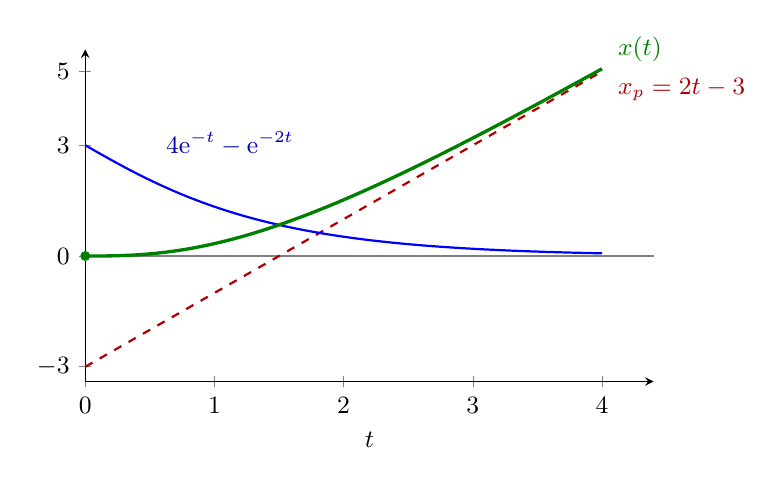
\begin{tikzpicture}[font=\small]
  \begin{axis}[
    axis lines=left, xmin=0, xmax=4.4, ymin=-3.4, ymax=5.6,
    xtick={0,1,2,3,4}, ytick={-3,0,3,5}, xlabel={$t$},
    width=8.8cm, height=5.8cm, clip=false, samples=100
    ]
    \draw[gray, thin] (axis cs:0,0) -- (axis cs:4.4,0);
    \addplot[red!70!black, thick, dashed, domain=0:4] {2*x-3};
    \addplot[blue, thick, domain=0:4] {4*exp(-x)-exp(-2*x)};
    \addplot[green!50!black, very thick, domain=0:4] {4*exp(-x)-exp(-2*x)+2*x-3};
    \fill[green!50!black] (axis cs:0,0) circle (1.8pt);
    \node[red!70!black, anchor=west] at (axis cs:4.05,4.5) {$x_p=2t-3$};
    \node[green!50!black, anchor=west] at (axis cs:4.05,5.6) {$x(t)$};
    \node[blue!70!black, anchor=south west] at (axis cs:0.55,2.45) {$4\mathrm{e}^{-t}-\mathrm{e}^{-2t}$};
  \end{axis}
\end{tikzpicture}
\end{document}
